%!TEX program = xelatex 
\documentclass[a4paper,zihao=-4]{article}
\usepackage[UTF8,punct,linespread=1.56]{ctex}
% \documentclass[a4paper,cs4size,UTF8,punct,linespread=1.56]{ctexart}
\pagestyle{empty} % 第二页以后页码空白
\usepackage[a4paper, left = 3.2cm, right = 3.2cm, top = 2.54cm, bottom = 2.54cm]{geometry}
\usepackage{xcolor}
% \usepackage[citebordercolor = white]{hyperref}
\usepackage[hidelinks]{hyperref}
\usepackage{graphicx} 
\usepackage{amsmath}
\usepackage{amssymb}
\usepackage{times}
\usepackage{multirow}
\usepackage[subrefformat=parens,labelformat=parens]{subfig} %
\usepackage{booktabs} % for \toprule \midrule \bottomrule \cmidrule
\usepackage{cleveref}
\crefformat{table}{表~#2#1#3 }
\crefformat{figure}{图~#2#1#3 }
\crefformat{equation}{式~(#2#1#3)}
\crefformat{chapter}{#2第#1章#3}
\crefformat{section}{#2第#1节#3}
\crefformat{subsection}{#2第#1节#3}
\crefformat{subsubsection}{#2第#1节#3}

\usepackage{tikz}
\usetikzlibrary{backgrounds,mindmap,calc,positioning,intersections}
\tikzstyle{startstop} = [rectangle, rounded corners, minimum width = 1cm, minimum height=0.5cm,text centered, draw = black]
\tikzstyle{io} = [trapezium, trapezium left angle=70, trapezium right angle=110, minimum width=1cm, minimum height=0.5cm, text centered, draw=black]
\tikzstyle{process} = [rectangle, minimum width=3cm, minimum height=1cm, text centered, draw=black]
\tikzstyle{decision} = [diamond, aspect = 3, text centered, draw=black]
% 箭头形式
\tikzstyle{arrow} = [->,>=stealth]

\usepackage{enumitem}
% \setenumerate[1]{itemsep = 0pt, parsep = 0pt, topsep = 2bp}
\setlist[enumerate]{itemsep = 0pt, parsep = 0pt, topsep = 2bp}
% \setitemize[1]{itemsep = 0pt, parsep = 0pt, topsep = 2bp}
\setlist[itemize]{itemsep = 0pt, parsep = 0pt, topsep = 2bp}
\usepackage{fontspec}
\setmainfont{Times New Roman}
% \usepackage{minted}   % For syntax highlighting
% \usemintedstyle{friendly}
\usepackage{setspace} 
\usepackage{caption}
\DeclareCaptionFont{capfont}{\kaishu\zihao{-4}\selectfont} % Caption font
\DeclareCaptionFont{subfont}{\kaishu\zihao{5}\selectfont} % Sub-caption font
\captionsetup{font = capfont}
\captionsetup[subfigure]{font = subfont}
\captionsetup[figure]{labelsep=space} % 空格 space;点 period;冒号 colon
\captionsetup[table]{labelsep=space}  % 空格 space;点 period;冒号 colon
\usepackage[square,numbers,sort&compress]{natbib}   % For Reference
\newcommand{\citess}[1]{\textsuperscript{\cite{#1}}}
\setlength{\bibsep}{1pt plus 0.3ex}
\usepackage{titlesec}
\titleformat{\subsubsection}[block]{\hspace{3em}}{\thesubsubsection}{1em}{}
\usepackage{insfc}



\graphicspath{{images/}}   % 设置图片所存放的目录

\begin{document}

\songti

% Decrease space above and below equations
\setlength{\abovedisplayskip}{0pt}
\setlength{\belowdisplayskip}{0pt}

%%%%%%%%% TITLE %%%%%%%%%
% \title{报告正文 \vspace{-3.4ex}}
% \title{报告正文}
% \maketitle
\begin{center}
	{\kaishu \zihao{3} \textbf{报告正文} \vspace{-3ex}}
\end{center}  

\thispagestyle{empty}    % 首页页码空白


{\kaishu \zihao{4}参照以下提纲撰写,要求内容翔实、清晰,层次分明,标题突出。}\alert{请勿删除或改动下述提纲标题及括号中的文字。\vspace{9bp}}

\NsfcChapter{(一)立项依据与研究内容}{\kaishu(建议8000字以内):}

\NsfcSection{1}{项目的立项依据}{(研究意义、国内外研究现状及发展动态分析,需结合科学研究发展趋势来论述科学意义;或结合国民经济和社会发展中迫切需要解决的关键科技问题来论述其应用前景。附主要参考文献目录);}

\subsection{研究背景和意义}
与中微子振荡相关的物理现象揭示了超出标准模型的新物理,是当前中微子物理研究的热点。在当前被广泛接受的三代中微子混合框架下,决定中微子振荡的参数包括两个质量平方差$\Delta m_{21}^2$和$\Delta m_{32}^2$,三个混合角$\theta_{12}$、$\theta_{23}$和$\theta_{13}$,以及CP破坏相角$\delta_{\text{CP}}$。其中,$\Delta m_{32}^2$的符号、$\theta_{23}$的卦限与$\delta_{\text{CP}}$都是尚未知的。如果$\theta_{13}$为0,那么由于其与$\delta_{\text{CP}}$在中微子振荡概率中的耦合关系,将无法通过振荡现象研究轻子的CP破坏。2012年,大亚湾反应堆中微子实验\citess{DayaBay:2012fng}首次以超过五倍标准偏差的显著度测量出$\theta_{13}$不为0。而且,测量出的$\theta_{13}$值比预期的要大,使得通过中微子振荡现象确定$\delta_{\text{CP}}$成为可能。此后,大亚湾实验一直提供了国际上最精确的$\theta_{13}$测量结果。\qiangdiao{当下,继续利用大亚湾实验未使用的大统计量数据的提高$\theta_{13}$的测量精度,对于这些中微子物理的未知量:$\Delta m_{32}^2$的符号、$\theta_{23}$的卦限与$\delta_{\text{CP}}$的探索将起到关键作用。}

\qiangdiao{\textbf{CP破坏相角与$\mathbf{\theta_{13}}$。}}CP对称性破缺在1964年被首次提出\citess{Christenson:1964fg}。CP破坏被认为是解释宇宙中正反物质不平衡现象的必要条件\citess{Sakharov:1967dj}。而中微子被认为是很可能揭开CP破坏起源之谜的粒子。目前,对轻子中的$\delta_{\text{CP}}$最好的限制结果来自日本的T2K实验\citess{T2K:2021xwb}和美国的NOvA实验\citess{NOvA:2021nfi}。它们的研究基于加速器中微子束流中的$\nu_\mu\to\nu_e$和$\overline{\nu}_\mu\to\overline{\nu}_e$振荡现象开展。T2K实验给出的最新结果是$\delta_{\text{CP}}$的值在最大CP破坏对应的$\pi/2$附近,$\delta_{\text{CP}}=0$和$\delta_{\text{CP}}=\pi$都在95\%的置信度下被排除。\qiangdiao{从\cref{tab:CP-measurements}进一步看出,使用反应堆中微子实验对$\theta_{13}$的精确测量结果,能大大提升T2K实验对$\delta_{\text{CP}}$的限制程度。NOvA实验则直接使用了反应堆中微子实验对$\theta_{13}$的精确测量结果,但其研究结果却受到$\theta_{23}$卦限假设的明显影响。}总结而言,给定质量次序和$\theta_{23}$卦限假设下,NOvA实验研究得到的90\%置信水平下的$\delta_{\text{CP}}$范围覆盖了所有可能的值,并未给出CP破坏存在与否的倾向。在未来实验中,更高的$\theta_{13}$精度和明确的$\theta_{23}$卦限对$\delta_{\text{CP}}$范围的进一步确定是关键的。
\begin{table}[htb!]
	\centering
	\setlength{\tabcolsep}{10pt}
	\zihao{5}
	\caption{T2K和NOvA实验对$\delta_{\text{CP}}$最新的限制结果和一倍标准偏差。其中,NO为正质量次序假设,IO为反质量次序假设。T2K only代表T2K实验不使用反应堆中微子实验对$\theta_{13}$的测量结果,T2K+Reactor则代表T2K实验使用反应堆中微子实验对$\theta_{13}$的测量结果来提升显著度。UO和LO代表$\theta_{23}$的不同卦限,分别对应于$\theta_{23}>45^\circ$和$\theta_{23}<45^\circ$.}
	\begin{tabular}{ccccc}
		\toprule
		\multirow{2}{*}{质量次序假设} & \multicolumn{2}{c}{T2K实验} & \multicolumn{2}{c}{NOvA实验} \\ 
		\cmidrule{2-3} \cmidrule{4-5}
	& \multicolumn{1}{c}{T2K only} & \multicolumn{1}{c}{T2K+Reactor} & \multicolumn{1}{c}{UO} & \multicolumn{1}{c}{LO} \\
		\midrule          
		NO & $-2.14^{+0.90}_{-0.69}$ & $-1.89^{+0.70}_{-0.58}$ & $2.58^{+0.85}_{-2.73}$ & $0.22^{+0.94}_{-0.82}$ \\
		IO & $-1.26^{+0.61}_{-0.69}$ & $-1.38^{+0.48}_{-0.55}$ & $4.78^{+0.85}_{-0.94}$ & $4.43^{+0.57}_{-0.69}$ \\
		\bottomrule
	\end{tabular}%
	\label{tab:CP-measurements}%
\end{table}%

\qiangdiao{\textbf{$\mathbf{\theta_{23}}$的卦限与$\mathbf{\theta_{13}}$。}}对$\theta_{23}$的测量主要是通过加速器中微子和大气中微子实验中$\nu_\mu\to\nu_\mu$和$\overline{\nu}_\mu\to\overline{\nu}_\mu$的振荡现象开展的。这两个振荡通道对应的概率近似为$1-\sin ^2 2 \theta_{23} \sin \left(\frac{\Delta m_{32}^2 L}{4 E}\right)$,其中$E$和$L$分别为中微子的能量和飞行距离。因此在有限的精度下,测量出$2\theta_{23}$接近于$90^\circ$,无法由此确定$2\theta_{23}>90^\circ$还是$2\theta_{23}<90^\circ$。通过加速器中微子和大气中微子实验中的$\nu_\mu\to\nu_e$和$\overline{\nu}_\mu\to\overline{\nu}_e$的振荡可以确定$\theta_{23}$卦限\citess{Agarwalla:2013ju}。该振荡主要的概率项为$\sin ^2 2 \theta_{13} \left(\sin ^2 \theta_{23} \sin ^2 \frac{\Delta m_{32}^2 L}{4 E}+ \cos ^2 \theta_{23} \sin ^2 \frac{\Delta m_{21}^2 L}{4 E}\right)$,其振幅与$\sin^22\theta_{13}$成正比。\qiangdiao{因此,$\sin ^2 2 \theta_{13}$的精度提升将直接降低该项振荡概率观测的不确定度,帮助$\theta_{23}$参数的确定。}

\qiangdiao{\textbf{中微子质量次序与$\mathbf{\theta_{13}}$。}}中微子质量次序的确定是粒子物理学和宇宙学的主要挑战之一,这不仅因为它能影响自然界质量产生的基本理论,而且能决定未来无中微子双$\beta$衰变实验的规模\citess{Gariazzo:2022ahe}。目前国际上的联合分析\citess{Esteban:2020cvm,Kelly:2020fkv}结果显示,数据更倾向于支持正质量次序(NO)而非反质量次序(IO)。目前,对中微子质量次序敏感的实验结果主要来自T2K实验\citess{T2K:2021xwb},NOvA实验\citess{NOvA:2021nfi},MINOS实验\citess{2018npa..confE.423A},Super-K实验\citess{Super-Kamiokande:2017yvm}和IceCube/DeepCore实验\citess{IceCube:2017lak}。未来的JUNO\citess{JUNO:2021vlw},Hyper-K\citess{Hyper-Kamiokande:2022smq}和DUNE\citess{DUNE:2020fgq}等实验都将提升对中微子质量次序的灵敏度。中微子质量次序可以通过几个GeV的大气中微子的能量和天顶角依赖性来确定。物质效应对振荡概率的影响可以使$\nu_\mu\to\nu_e$的振荡在NO假设下增强,而使$\overline{\nu}_\mu\to\overline{\nu}_e$的振荡在IO假设下增强。加速器实验也可以基于相同的效应探索中微子的质量次序。比如,这一效应可以使NOvA实验观测到的振荡概率改变约20\%\citess{NOvA:2021nfi}。\qiangdiao{与$\theta_{23}$卦限的确定类似,$\nu_\mu\to\nu_e$和$\overline{\nu}_\mu\to\overline{\nu}_e$的振荡概率主要项都与$\theta_{13}$有关。$\theta_{13}$精度的提升对这些中微子物理未知参数的确定都具有重要意义。}

\subsection{国内外研究现状及分析}
国际上对$\theta_{13}$灵敏度最高的实验主要是短基线反应堆中微子实验,包括中国的大亚湾实验\citess{DayaBay:2022orm},韩国的RENO实验\citess{RENO:2018dro}和法国的Double Chooz实验\citess{DoubleChooz:2019qbj}。2012年,大亚湾实验\citess{DayaBay:2012fng}首次以超过五倍标准偏差的显著度测量出$\theta_{13}$不为0,发现了新的中微子振荡模式,之后被RENO实验\citess{RENO:2012mkc}和Double Chooz实验\citess{DoubleChooz:2012gmf}确认。

大亚湾实验于2011年12月24日开始采数,2020年12月12日停止采数。RENO实验于2011年8月11日开始采数,目前仍在运行。Double Chooz实验于2015年1月开始以多个探测器开始运行采数,2017年12月份停止采数。\qiangdiao{三个实验中,大亚湾实验使用八个全同设计的探测器收集来自六个最高热功率为2.9 GW的反应堆释放出的$\overline{\nu}_e$信号,具有最高的统计量,也因此提供了国际上最高精度的$\theta_{13}$测量结果。}

这三个实验组除了使用本底较少的钆俘获样本开展$\theta_{13}$测量\citess{DoubleChooz:2014kuw}之外,\qiangdiao{还使用了统计和系统误差独立的氢俘获样本研究来提供交叉检验}。Double Chooz实验还于2020年发表了全中子俘获样本联合的分析结果\citess{DoubleChooz:2019qbj},以进一步提高测量精度。除了这三组实验外,加速器中微子实验和大气中微子实验也可以利用$\nu_\mu\to\nu_e$和$\overline{\nu}_\mu\to\overline{\nu}_e$的振荡对$\theta_{13}$进行测量,但其灵敏度远不如反应堆实验。如\cref{fig:world-status},展示了国际上各种实验提供的$\theta_{13}$测量结果,同时展示的是对质量平方差$\Delta m_{32}^2$的测量结果。其中,黑色点展示的是大亚湾实验3158天的完整钆俘获样本测量结果\citess{DayaBay:2022orm},已提交到预印本网站\texttt{arxiv.org}上;红色点展示的是基于大亚湾实验1958天采集的氢俘获样本研究的测量结果,已完成合作组内部分析评审。
\begin{figure}[!htb]
    \centering
    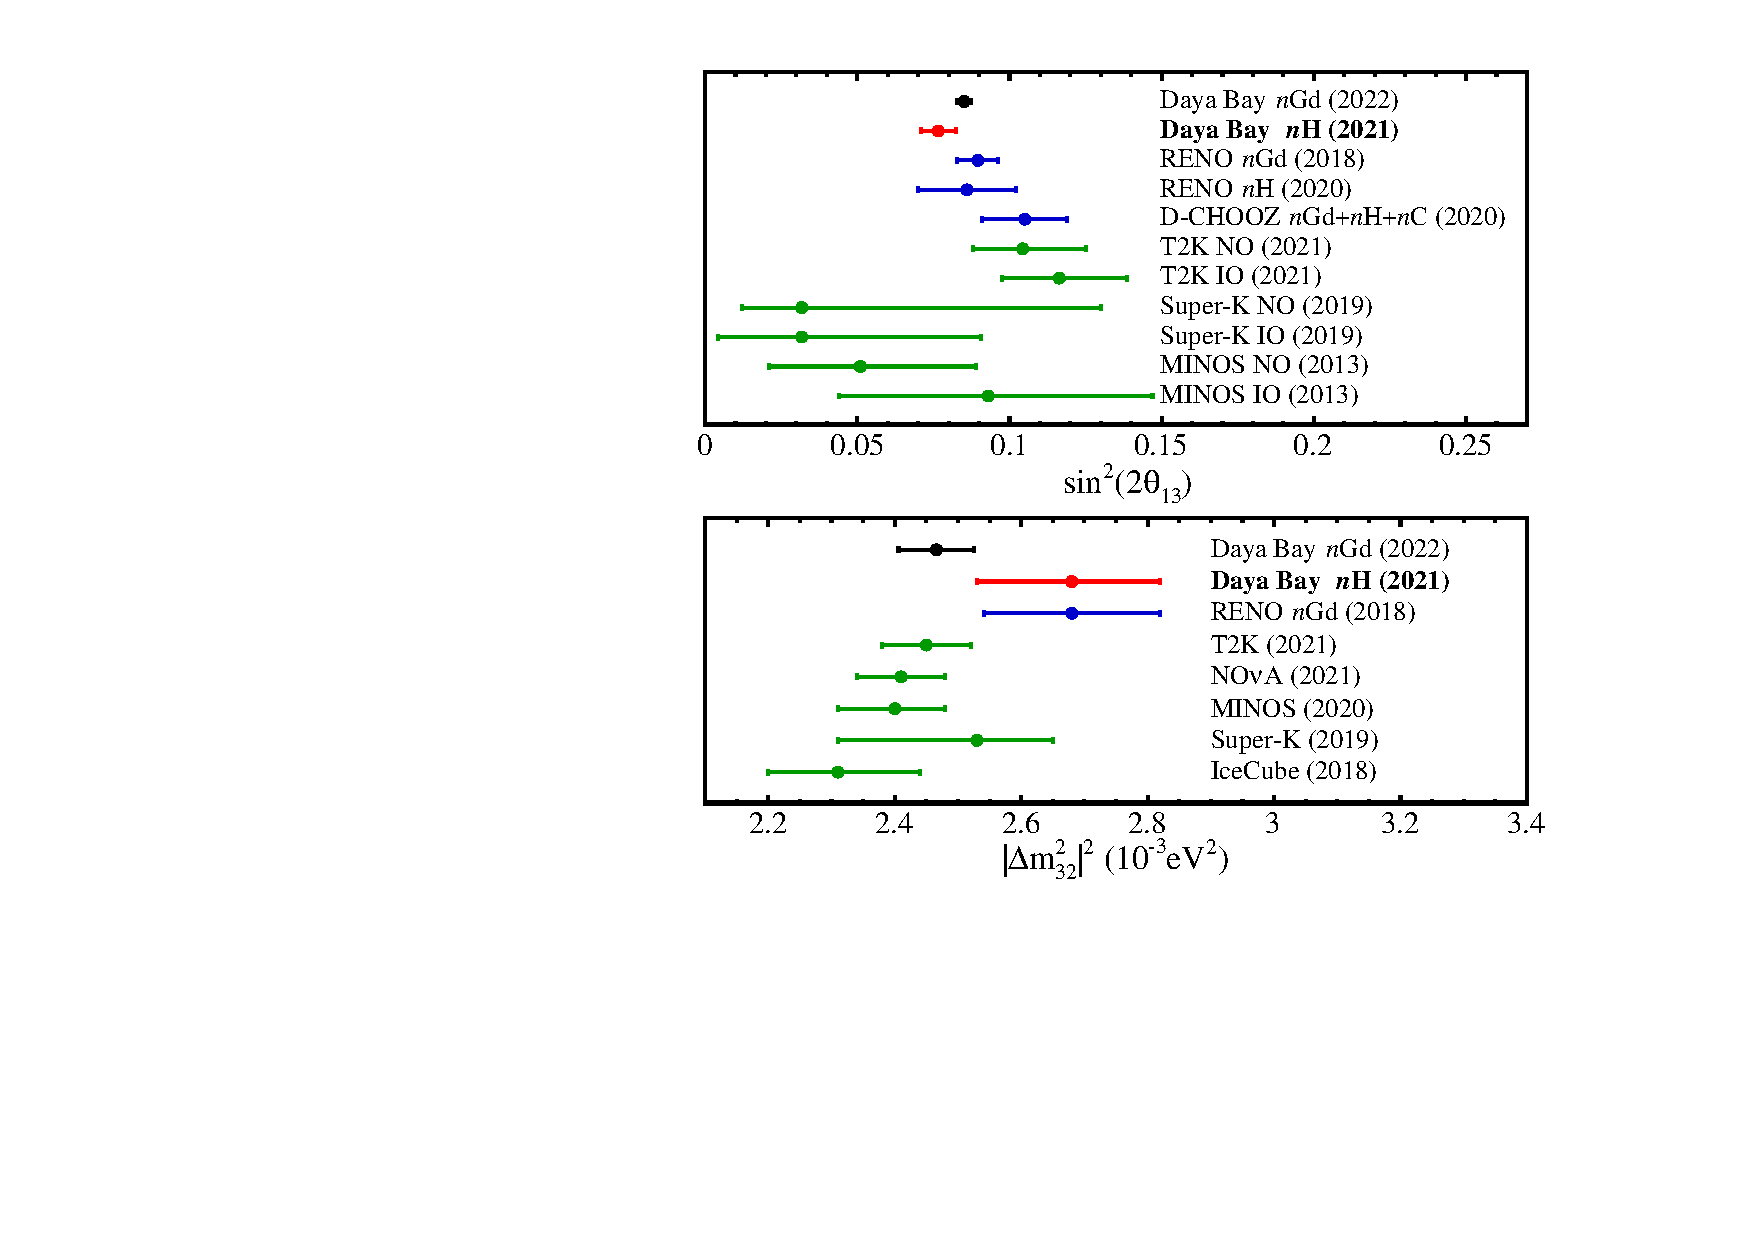
\includegraphics[width=15cm]{WorldMeas.pdf}
    \caption{世界上各种实验对$\sin^22\theta_{13}$(上图)和$\Delta m_{32}^2$(下图)的测量结果比较。其中NO代表正质量次序假设,IO代表反质量次序假设。此处展示的$\sin^22\theta_{13}$测量值取自大亚湾实验钆俘获样本测量\citess{DayaBay:2022orm}(黑点)、大亚湾实验氢俘获样本测量(红点)、RENO实验钆俘获样本测量\citess{RENO:2018dro}(蓝点)、RENO实验氢俘获样本测量\citess{RENO:2019otc}(蓝点)、Double Chooz实验全中子俘获样本测量\citess{DoubleChooz:2019qbj}(蓝点)、T2K实验NO和IO假设\citess{T2K:2021xwb}(绿点)、超级神冈实验NO和IO假设\citess{Super-Kamiokande:2019gzr}(绿点)、MINOS实验NO和IO假设\citess{MINOS:2013xrl}(绿点);$\Delta m_{32}^2$测量值取自大亚湾实验钆俘获样本测量\citess{DayaBay:2022orm}(黑点)、大亚湾实验氢俘获样本测量(红点)、RENO实验钆俘获样本测量\citess{RENO:2018dro}(蓝点)、T2K实验\citess{T2K:2021xwb}(绿点)、超级神冈实验\citess{Super-Kamiokande:2019gzr}(绿点)、MINOS实验\citess{MINOS:2020llm}(绿点)和IceCube实验\citess{IceCube:2017lak}(绿点)。$\Delta m_{32}^2$测量值都是NO假设下的结果,IO假设下的比较与之类似,此处不再展示。其中大亚湾实验2021年完成的氢俘获样本研究仅使用了1958天采取的数据。}
    \label{fig:world-status}
\end{figure}

\subsection{项目研究动机}
大亚湾实验,RENO实验和Double Chooz实验提供的最精确的$\sin^22\theta_{13}$测量精度分别为2.8\%,7.6\%和13\%。前两个结果都是基于钆俘获样本的研究。此外,大亚湾实验还有能力进一步提高测量精度。\qiangdiao{大亚湾实验新近完成合作组评审的基于62\%氢俘获样本研究的$\sin^22\theta_{13}$测量精度已经达到RENO最新钆俘获样本研究的精度。与大亚湾完整数据集相比,还有1200天的数据未参与研究。因此,基于大亚湾氢俘获样本研究的$\theta_{13}$测量精度还有很大的提升空间。}

本项目旨在通过联合氢俘获和钆俘获数据集的$\sin^22\theta_{13}$测量结果,给出国际上最精确的测量值。目前,完整钆俘获数据集的研究已经完成,使用62\%的氢俘获数据集的工作也已完成。延续这些工作,本项目将完成下述物理目标:
\begin{enumerate}
	\item 使用完整氢俘获样本完成$\theta_{13}$测量。\qiangdiao{不仅基于统计上的显著提升,也将通过系统误差的显著压低提升测量精度。}\qiangdiao{预期此项分析将给出国际上第二精确的$\theta_{13}$测量结果,精度约6\%}。本项目预期将此项结果对最终联合结果贡献的权重因子从之前的16\%提高到约30\%。
	\item 将完整氢俘获数据样本的研究结果与已公开的完整钆俘获数据样本的研究结果\citess{DayaBay:2022orm}进行联合,\qiangdiao{给出大亚湾实验最终的$\theta_{13}$测量结果,将其2.8\%的测量精度改进到约2.5\%}。
\end{enumerate}

\begin{spacing}{1.3} % 行距
	\zihao{5} \songti   
	\bibliographystyle{apsrev4-1}
	\bibliography{ref}  
	\vspace{11bp}
\end{spacing}

\NsfcSection{2}{项目的研究内容、研究目标,以及拟解决的关键科学问题}{(此部分为重点阐述内容);}

\subsection{研究目标}
本项目的研究依托于自2011年12月24日便开始运行的大亚湾反应堆中微子实验,预期完成以下研究目标。
\begin{itemize}
	\item \qiangdiao{目标一:} 基于3158天的氢俘获数据样本,重新完成$\overline{\nu}_e$信号选择、偶然符合本底的估计、快中子本底的估计、$^9$Li/$^8$He本底的估计、放射性中子本底的估计,\qiangdiao{并开展新的muon-x本底的研究。预期将$^9$Li/$^8$He本底事例率的估计精度从约50\%提升至约30\%。}
	\item \qiangdiao{目标二:}基于更高统计量的数据,开展探测器一致性检查,基于此进一步完善快信号能量、慢信号能量以及距离时间选择效率的系统误差研究。
	\item \qiangdiao{目标三:}使用新的能量非线性数据,更新探测器能量响应模型,并基于该模型开展新的探测器相关的能谱系统误差研究。
	\item \qiangdiao{目标四:}将完整数据集的氢俘获研究和钆俘获研究的振荡分析结果联合,\qiangdiao{预期氢俘获研究单独的$\sin^22\theta_{13}$测量精度从7\%提升至6\%,联合研究将使钆俘获分析的$\sin^22\theta_{13}$测量精度提升到约2.5\%。}
\end{itemize}

\subsection{研究内容}

为了完成上述研究目标,本项目的研究内容主要分为以下四个部分:
\begin{enumerate}
	\item \qiangdiao{氢俘获样本的本底分析。}该项内容具体可分为偶然符合本底、宇宙射线导致的本底和探测器材料中的放射性中子本底的分析与含量估计。本项目将重点完善宇宙射线相关本底的估计方法,并改进估计精度。
	\item \qiangdiao{探测器一致性检查和探测效率系统误差分析。}该项内容基于数据完成探测器间的比较和一致性检验,进而完成快慢信号的能量选择效率,时间间隔与距离选择效率对应的系统误差分析。
	\item \qiangdiao{探测器能量响应模型的优化。}
	\item \qiangdiao{氢俘获样本研究结果与钆俘获样本研究结果的联合。}
\end{enumerate}
	
以下\cref{sec:backgrounds}至\cref{sec:nGdnH-combine}将对这些内容展开讨论。为便于理解本项目的具体研究内容,\cref{sec:dayabay-basic}对与本项目相关的大亚湾实验的基本信息进行简要总结。

\subsubsection{与本项目相关的大亚湾实验的基本信息总结}\label{sec:dayabay-basic}
实验前后在三个实验厅(EH1,EH2和EH3)共安装有八个全同设计的探测器,用于探测大亚湾、岭澳一期和岭澳二期共六个核电反应堆释放出的电子反中微子。实验厅EH1的两个探测器(EH1-AD1和EH1-AD2)与大亚湾反应堆距离约360 m,EH2的两个探测器(EH2-AD1和EH2-AD2)与岭澳一期和岭澳二期反应堆相距约500 m。在这种距离下,反应堆释放出的电子反中微子 ($\overline{\nu}_e$) 的振荡效应极其微小,故而可以对反应堆中微子的流强进行精确测量。EH3的四个探测器(EH3-AD1,EH3-AD2,EH3-AD3和EH3-AD4)与大亚湾和岭澳反应堆的距离分别约为1.9 km和1.5 km。在这一飞行距离下,$\overline{\nu}_e$存活几率中与$\Delta m_{31}^2$/$\Delta m_{32}^2$相关的振荡项成为主导,其对应的振幅近似由$\sin^22\theta_{13}$决定,如\cref{eq:oscillation-prob}所示。
\begin{equation}\label{eq:oscillation-prob}
	\begin{aligned}
P_{\text {sur }}= & 1-\cos ^4 \theta_{13} \sin ^2 2 \theta_{12} \sin ^2 \Delta_{21} \\
& -\sin ^2 2 \theta_{13}\left(\cos ^2 \theta_{12} \sin ^2 \Delta_{31}+\sin ^2 \theta_{12} \sin ^2 \Delta_{32}\right),
\end{aligned}
\end{equation}
其中$\Delta_{j i} \simeq 1.267 \Delta m_{j i}^2\left(\mathrm{eV}^2\right) L(\mathrm{~m}) / E_\nu(\mathrm{MeV})$. 

探测器为柱形设计。其最中心是20吨掺钆液体闪烁体(GdLS),被直径和高度均为3 m的亚克力容器(IAV)容纳。外部被容纳在直径和高度均为4 m的亚克力容器(OAV)中的约 22 吨不掺钆的液体闪烁体 (LS)包裹着。LS原本设计为钆俘获数据研究中的的能量收集器,后也被氢俘获数据研究作为最主要的靶物质。这些结构都被沉浸在最外部直径和高度均为5 m的不锈钢容器中的原油中,以保护GdLS和LS免受外部材料辐射的影响。为了降低宇宙线对中心探测器的影响,同一个实验厅的探测器被沉浸于水池中,其外部组成水切伦科夫探测器以对宇宙线进行反符合。

探测器在柱形探测器的SSV桶壁内侧安装了192 个 20-cm 光电倍增管(PMT),以探测器GdLS和LS中形成的闪烁光。当$\overline{\nu}_e$穿过探测器,有一定概率与探测器中的质子发生反$\beta$衰变反应(IBD)。如\cref{eq:IBD}所示,IBD反应末态会生成两个粒子:正电子和中子。
\begin{equation}\label{eq:IBD}
	\overline{\nu}_e+p\to e^++n
\end{equation}
正电子如果穿过GdLS和LS区域,其损失的能量会被转化为闪烁光光子。闪烁光光子击中PMT光阴极,就会被转化为电信号被记录下来。而中子则首先被慢化,然后会被核俘获,继而俘获核释放出$\gamma$被探测到。在实验中,中子主要被钆核和氢核所俘获,对应的释放出$\gamma$的时间分别约为30 $\mu$s和200 $\mu$s。因此,IBD信号的一大特征是正电子形成的快信号与中子俘获形成的慢信号在时间上的符合,这一特征将$\overline{\nu}_e$信号与大部分本底明显地区分开来。

中子被钆核俘获对应的IBD数据样本被称为钆俘获样本($n$Gd-IBD),该样本通过钆核释放出的总能量约8 MeV的几个$\gamma$来标记。由于该特征能量很高,$n$Gd-IBD的研究受本底的影响很小。中子被氢核俘获对应的IBD数据样本被称为氢俘获样本($n$H-IBD),该样本通过氢核释放出的单个2.2 MeV的$\gamma$来标记。由于2.2 MeV附近存在很多放射性活动形成的本底,$n$H-IBD样本的研究受本底影响较大。在远厅EH3的探测器中,$\overline{\nu}_e$信号数与本底数接近$1:1$,这是造成本项目研究难点的主要根源。

借助于远近点共八个全同设计的探测器,大亚湾实验可以进一步摆脱反应堆关联和探测器间关联的系统误差的影响,与之前的实验相比可以显著提升测量精度。实验中占主要贡献的系统误差均为探测器间非关联的,这一类系统误差的表现是八个探测器上的差异性。实验采用数据对八个探测器的各种表现进行比对,确定探测器间的差异,以此估计系统误差。

\subsubsection{氢俘获样本的本底分析}\label{sec:backgrounds}
根据快慢信号在时间上的关联性,利用固定时间窗内的事例符合可以筛选出数据中的$\overline{\nu}_e$信号。快信号的能量被要求在$[1.5, 12]$ MeV,慢信号的能量则处于2.2 MeV附近。该能量范围与很多放射性活动的低能本底有重叠。这些本底基本是单事例,少数的级联衰变本底如$^{214}\text{Bi}-^{214}\text{Po}-^{210}\text{Pb}$和$^{212}\text{Bi}-^{212}\text{Po}-^{208}\text{Pb}$形成的$\beta$-$\alpha$快慢信号已被能量筛选条件排除掉。两个单事例随机组合有概率满足时间符合条件,如果进一步满足$\overline{\nu}_e$信号的其他筛选条件,就形成了偶然符合本底。偶然符合本底的事例率与单事例率、符合时间长度和宇宙线缪子反符合率有关,在理论上可以被精确估计,其误差可以忽略。

宇生本底主要包括快中子本底和$^9$Li/$^8$He本底,除此之外还包含了实验末期数据采集过程中由于水池对宇宙线反符合效率下降而引发的的新muon-x本底。
\begin{itemize}
	\item $^9$Li/$^8$He本底。宇宙线缪子及其散裂产物可以与有机液闪中的$^{12}$C发生强和电磁相互作用,产生中子和新的同位素。在这些宇生同位素中,$^9$Li 和 $^8$He 可以通过$\beta^-$衰变转变为一个不稳定的核素,然后立即释放出一个中子。这样的 $\beta$-n 级联衰变就可以构成与 IBD类似的快慢信号。$^9$Li 和 $^8$He 的寿命分别约为 257 ms 和 172 ms,这比实验中对绝大部分缪子的反符合时间都要长。除此之外,它们的快信号 $\beta$ 的能量最高可以达到 13.6 MeV,与 IBD 事例的快信号能量有很大一部分交叠,故而能形成IBD候选事例中的本底。
	\item 快中子本底。宇宙线缪子还可以生成高能的散裂中子。后者在进入到探测器的过程中被慢化,会留下反冲信号作为快信号,然后被俘获从而留下中子俘获的慢信号。以这种方式,快中子通过质子反冲和中子俘获构成的快慢信号被筛选进 IBD 候选事例中。探测器外部水池对宇宙线缪子具有很高的标记效率,并且对在探测器中留下能量的缪子反符合时间较长,因此在探测器内部形成的快中子基本无法被筛选进信号样本中。但宇宙线缪子在水池外部的岩石中形成的快中子却可以逃过反符合系统。从外部而来的快中子形成的本底事例更多地集中在 LS 区间,因而快中子本底对$n$H分析的影响比对$n$Gd分析更大。
	\item \qiangdiao{muon-x本底。实验末期,由于水池顶部附近PMT的性能逐渐下降,外水池的宇宙线缪子反符合效率随时间下降。一些低能的缪子可以穿过水池而不被探测到。缪子形成的快信号,与缪子衰变产生的Michel电子或者散裂中子形成的慢信号一起构成了快慢事例对。}
\end{itemize}

放射性中子主要是通过核素自发裂变和$(\alpha,n)$反应产生的。这两个过程在产生中子的同时,还会产生伴随的$\gamma$。如果探测器的靶物质外部的屏蔽材料不够厚,这些中子和$\gamma$就可以进入到中心的液闪区域并沉积能量。中子的反冲信号和$\gamma$可以形成快信号,中子被俘获然后释放出的$\gamma$可以形成慢信号,这样就构成了具有 IBD 信号特征的本底事例。核素的每次自发裂变一般会同时产生多个$\gamma$和中子,因此除了以$(\alpha,n)$类似的机制形成本底外,还可以通过多个中子俘获之间的符合形成本底。

除了上述本底外,还有探测器顶部的Am-C刻度源形成的中子本底。该本底通过之前的研究已经得到妥善的估计,并且在本底中占比极少,因而不需要在本项目中进行完善。

\subsubsection{探测器一致性检查和探测效率的系统误差研究}\label{sec:uncertainty}
对基于事例率的振荡分析而言,每一项会影响探测器收集到的IBD事例数的因素都会贡献一项系统误差。从反应堆流强出发,一个大亚湾探测器探测到的信号数可以由\cref{eq:signal-number}预测。
\begin{equation}\label{eq:signal-number}
	N_{\text{sig}} = \phi_{\text{eff}} \times \varepsilon_\mu\varepsilon_m\left(\sum_{v}N_{p,v}\varepsilon_{e,v}\right)\varepsilon_{\text{DT}}
\end{equation}
其中,
\begin{itemize}
	\item $v$代表不同靶材料。对于本项目而言,主要包括GdLS、LS、IAV和OAV。
	\item $\phi_{\text{eff}}$是从反应堆到达探测器的有效$\overline{\nu}_e$数目,包含了反应堆释放出的中微子数目、IBD反应的界面、从反应堆到探测器的距离和振荡参数等因素的影响。除了从反应堆到探测器的距离对八个探测器存在差异外,其余因素都对每个探测器的$N_{\text{sig}}$影响相同。而且基线的测量精度很高,在实验中可以忽略。所以,$\phi_{\text{eff}}$可以直接借用之前氢俘获分析的结果,不是本项目的研究内容。
	\item $\varepsilon_\mu$是对数据进行离线宇宙线反符合之后,数据的存留效率。$\varepsilon_m$是受单事例本底影响下,在数据中IBD信号形成快慢事例对的效率。这两项效率都可以利用数据进行精确测量,其误差可以忽略。故而本项目可以直接沿用之前的方法进行更新,也不是重点研究内容。
	\item $N_{p,v}$是靶材料$v$的质子数。实验提供了每部分靶材料的质量测量值和误差,可以用于计算质子数及其误差。因而,该项可以直接参考之前氢俘获分析的计算结果,不需重复研究。
	\item $\varepsilon_{e,v}$代表对每项靶材料不同的效率,主要包含快信号的能量选择效率和慢信号的能量选择效率。该项的系统误差在以往分析中占主要部分,可以使用更高统计量的数据开展更完善的研究,是本项目的重点研究内容。
	\item $\varepsilon_{\text{DT}}$是对整个探测器内信号而言的距离时间联合选择效率。该项的系统误差在以往分析中的误差占比也是较为显著的,也是本项目的重点研究内容。
\end{itemize}

实验对快信号的能量选择范围为$[1.5, 12]$ MeV,对慢信号的能量选择范围是$[\mu-3\sigma, \mu+3\sigma]$。其中,$\mu$是每个探测器各自拟合出的IBD氢俘获的能量峰位,$\sigma$则为该能量蜂的高斯分布标准差。为了保证使用这套选择条件对每个探测器都可以获得相同的效率,必须检查每个探测器的能标和分辨率差异,并使用模拟的IBD样本将能标的和分辨率的差异传递为选择效率的差异。最终这样得到的选择效率就作为其系统误差。

在以往分析中,距离时间联合选择效率都是通过每个探测器的数据进行估算的。实验可以放宽距离时间的选择条件,从而得到IBD信号完整的距离时间联合分布。通过计算该分布中选择条件以内的信号数占比,就可以估算$\varepsilon_{\text{DT}}$。进一步比较该占比在八个探测器间的差异,就可以估计出$\varepsilon_{\text{DT}}$的系统误差。

\subsubsection{探测器能量响应模型的优化}\label{sec:energy-model}
为了研究中微子振荡效应对中微子能量$E_\nu$的依赖,必须将实验中探测到的IBD快信号能谱与理论预测的能谱进行比较。探测器能量响应模型正是从中微子原始能量出发,考虑IBD末态正电子和中子在GdLS、LS以及其余不发光材料中的能量沉积,并在其基础上施加液闪发光非线性和电子学非线性的影响,接着基于实验观测数据考虑能量分辨率和空间非均匀性的影响,最终计算出理论上的IBD快信号能量。其中,液闪非线性主要是电离淬灭和切伦科夫光导致的,前者可以使高电离密度粒子的光产额降低,比如质子、$\alpha$粒子和低能$e^\pm$,后者则可以在粒子超过液闪中光的相速度的情况下使光产额增加,从而使沉积能量和可见光能量不成正比。电子学非线性则是由于探测到光子的时间分布和电子学读出系统的采集效率对电荷重建结果的影响引发的。

本项目将使用该能量响应模型建立中微子能量与IBD快信号能量的转换关系。该能量转换关系对于完成基于事例率和能谱的中微子振荡振幅和频率测量是必须的。然后使用该模型将上述各种探测器效应拆分开来,研究每一项因素对IBD能谱的影响,开展能谱相关的系统误差研究。

\qiangdiao{相比于目前氢俘获分析已有的能量响应模型,本研究将根据完整数据集提取出新的能量非线性曲线从而更新该响应模型,进而开展能谱相关的系统误差研究。}

\subsubsection{氢俘获样本研究结果与钆俘获样本研究结果的联合}\label{sec:nGdnH-combine}
\qiangdiao{由于氢俘获样本和钆俘获样本在统计和系统上都具有明显的独立性,将二者的分析结果联合将会提高大亚湾实验对$\theta_{13}$的测量精度。}

\qiangdiao{为了完成这一联合分析,关键任务是研究两个分析的关联性。}关联性按照来源可以分为:探测效率,IBD能谱,本底和反应堆相关的因素。其中反应堆相关的因素对于两个分析是完全关联的。两个分析虽然具有显著不同靶体积和选择条件,本底的成分也极为不同,但能量测量手段、本底分析方法和能量非线性等因素都具有关联性。\qiangdiao{根据之前的分析,基于事例率的氢俘获分析结果与基于事例率和能谱的钆俘获分析结果之间的相关系数仅为2\%。} 新的氢俘获分析引入了新的本底:放射性中子本底,还开展了基于能谱的振荡参数测量。这些因素使得两个分析的相关性进一步减弱。\qiangdiao{本项目将进一步对基于事例率和能谱的氢俘获分析结果和钆俘获分析结果之间的关联性进行研究,完成两个结果的联合。}

\subsection{拟解决的关键科学问题}
\qiangdiao{本项目将解决两个关键科学问题:A. 使用氢俘获数据集完成基于事例率和能谱的中微子振荡振幅和频率的测量;B. 联合氢俘获数据和钆俘获数据对振荡参数的测量结果。}

\qiangdiao{A问题在大亚湾实验,RENO实验和Double Chooz实验已发表的氢俘获数据研究结果中都尚未实现。}该问题的困难性在于氢俘获数据中的$\overline{\nu}_e$信号主要来自探测器靠外的靶材料中,能量泄露效应明显、本底高和系统误差显著等因素都造成其IBD能谱难以预测。立足于本项目的研究目标,这一科学问题的解决具有充分的条件。

\qiangdiao{B问题立足于A问题之上,是大亚湾实验主要物理目标的最终实现,旨在充分利用大亚湾实验相比于其他实验的优势,进一步提升$\theta_{13}$的测量精度,对未来中微子未知参数的探索具有重要意义。}

\NsfcSection{3}{拟采取的研究方案及可行性分析}{(包括研究方法、技术路线、实验手段、关键技术等说明);}
\subsection{研究方案}
\begin{figure}
  \centering
  \resizebox{1.0\textwidth}{!}{
    \begin{tikzpicture}[node distance=5em, text width=5em]
      %定义流程图具体形状+        \small
      \node[startstop](data){大亚湾实验重建数据};
      \node[startstop, right of = data, xshift=3em](candidates){$\overline{\nu}_e$候选事例样本};
      \node[startstop, right of = candidates, xshift = 3em](bkgsub){关联$\overline{\nu}_e$候选样本};
      \node[startstop, right of = bkgsub,xshift = 3em](ADcheck){探测效率及其系统误差};
      \node[startstop, right of = ADcheck,xshift = 3em](shapeuncer){能谱预测及其系统误差};
      \node[startstop, below of = bkgsub](corrbkg){关联本底};
      \node[startstop, below of = shapeuncer](nHresult){$n$H样本振荡分析结果};
      \node[startstop, below of = nHresult](combine){$n$H和$n$Gd结果合并};
      %连接具体形状
      % \draw (dec1) -- node [above] {N} (point1);
      \draw [arrow] (data)  -- node [above, yshift=1.3em] {时间符合} (candidates);
      \draw [arrow] (candidates)  -- node [above, yshift=1.3em, text width=5em,align=center] {扣除偶然符合本底} (bkgsub);
      \draw [arrow] (bkgsub)  -- node [above, yshift=1.3em, text width=8em,align=center] {探测器一致性检查和模拟数据研究} (ADcheck);
      \draw [arrow] (bkgsub)  -- node [left, text width=14em, yshift=-0.5em, align=center] {宇生本底和放射性中子本底估计} (corrbkg);
      \draw [arrow] (corrbkg)  -- node [above, yshift=0.2em, text width=5em,align=center] {建立$\chi^2$} (nHresult);
      \draw [arrow] (ADcheck)  -- node [above, yshift=1.3em, text width=5em,align=center] {能量响应模型} (shapeuncer);
      \draw [arrow] (shapeuncer)  -- node [above, yshift=-0.65em, text width=5em,align=center] {} (nHresult);
      \draw [arrow] (nHresult)  -- node [left, xshift=1.45em, yshift=-0.2em, text width=15em,align=center] {$n$H与$n$Gd研究结果的关联性分析} (combine);
    \end{tikzpicture}
  }
  \caption{本项目拟议的技术路线图。方框中的文字描述了重要节点对应的研究结果,箭头上的文字说明了关键技术。}
  \label{fig:CalibrationProce}
\end{figure}

本项目的原始数据是大亚湾实验从2011年12月24日至2020年12月12日共运行3158天采集的数据,目前已由合作组成员完成刻度与事例重建。本项目将主要运用CERN提供的大数据分析软件包ROOT对采集的事例进行关联性分析并去除本底以获得干净的$\overline{\nu}_e$信号,并使用探测器模拟软件包GEANT4完成部分探测效率和系统误差研究,最后利用ROOT极小化带有pull-term的$\chi^2$来得到最优振荡参数。

\cref{fig:CalibrationProce}展示了本项目拟议的技术路线图,其中方框表明了重要研究节点对应的分析结果,箭头上的说明文字表示为了得到该研究结果所需实现的实验手段。

从大亚湾实验的重建数据出发,本项目将分析重建事例之间的时间关联性,利用事例在固定时间窗的符合得到快慢事例对,即构成了$\overline{\nu}_e$候选事例样本。基于候选事例中的单事例统计结果完成偶然符合本底的估计,并将该本底从候选事例中扣除,就得到了关联$\overline{\nu}_e$候选样本。该关联候选样本主要包含了宇生本底和放射性中子本底。对于放射性中子本底,项目团队已有成熟的理论计算和探测器模拟模型对其进行研究。宇生本底则包含了快中子本底、$^9$Li/$^8$He本底和实验末期才出现的muon-x本底,这些本底都需要根据其特征进行单独的研究。\qiangdiao{快中子本底和$^9$Li/$^8$He本底已有成熟的分析方案,后者预期可以通过提高其分析方法中的能量选择阈值而获得更好的估计精度。muon-x本底的分析方法则可以借鉴快中子本底,并根据其来源不同进行调整,在合作组内已有在$n$Gd样本上的成功实践可以参考。}完成了这些,就得到了总的$\overline{\nu}_e$候选事例样本、关联$\overline{\nu}_e$候选样本和本底估计结果。

关联$\overline{\nu}_e$候选样本中的本底占比极少,可以基于该样本开展探测器一致性检查。检查的重点是八个探测器的能标、分辨率、信号能谱和距离时间联合分布的差异。对这些差异的确定将提供探测器间非关联变化的量化估计,进而联合模拟数据研究估计出这些差异对应的探测效率变化。将检查结果与根据实验最新的非线性数据更新后的探测器能量响应模型结合,可以预测IBD能谱并估计各项探测器相关的因素可能对能谱导致的系统误差。

将候选事例样本和本底评估的统计结果输入到$\chi^2$,并以pull-term的形式考虑进探测效率和能谱的系统误差项的影响,然后保持振荡参数$\sin^22\theta_{13}$和$\Delta m_{32}^2$为自由参数将$\chi^2$极小化,就得到了$n$H-IBD样本的振荡分析结果。

$n$Gd-IBD样本的研究结果已经公布。\qiangdiao{对$n$H-IBD分析中$\chi^2$的每个系统误差项与$n$Gd-IBD分析中对应项的关联性进行分析,并得到总体上两个分析的相关系数,}就可以对$n$Gd于$n$H分析结果进行合并,\qiangdiao{达到提升精度后的结果}。关联性的分析将对每个系统误差项的物理来源、估计方法与估计结果展开。

上述路线图中可能的难点与预期解决方案如下。
\begin{itemize}
	\item \qiangdiao{难点一:}对$^9$Li/$^8$本底事例率的评估精度提升的预期可能因统计量不足受限。本项目计划参考$n$Gd分析,将$^9$Li/$^8$He本底样本的快信号能量筛选条件从3.5 MeV提升至8 MeV,以提高$^9$Li/$^8$He在该样本中的信噪比,从而提高估计的精度。但提高能量阈值后,整体样本的统计量会下降。$^9$Li/$^8$He含量的估计是通过拟合事例相距缪子的时间分布,而统计量降低会使该拟合容易失败。预期,优化$^9$Li/$^8$He能量阈值以平衡统计量与信噪比的关系,并优化时间谱拟合的条件,可以妥善解决此问题。
	\item \qiangdiao{难点二:}在评估系统误差时需要比较和理解不同样本呈现出的探测器一致性的差异,并可能需要对非IBD样本的研究结果进行修正。比如,研究能标和能谱在探测器间的差异会着重参考IBD样本和散裂中子样本呈现的结果,这是因为两个样本的高度相似性。但是后者与宇宙线有关,在三个实验厅的具体性质存在差异,这一特性对探测器差异研究结果的影响需要仔细考虑。再比如,比较距离时间联合分布在探测器间的差异时会着重参考IBD样本和$^{214}$Bi-$^{214}$Po样本,也是因为两个样本的相似性。但对于二者不同之处可能需要修正,而修正可能存在一定困难。因为IBD样本主要分布在LS区间,$^{214}$Bi-$^{214}$Po样本虽在LS区间也有分布但主要还是集中在GdLS区域。按照探测器不同区域将$^{214}$Bi-$^{214}$Po样本的距离时间分布按照IBD样本进行归一化修正时,LS边界处的$^{214}$Bi-$^{214}$Po过低的统计量会影响修正效果。预期,结合完整数据更大的统计量,尝试多种修正方法和使用多种参考样本来给出一致的系统误差评估结果,能够解决这一问题。
	\item \qiangdiao{难点三:}根据$n$Gd和$n$H分析的各项系统误差的关联性导出两个结果整体关联性时,与能谱相关的关联性可能需要额外考量。在之前基于事例率的分析中,只有探测效率和本底估计会影响信号事例数,而反应堆相关的项对两个分析是完全关联的。在本项目的基于事例率和能谱的分析中,振荡参数$\sin^22\theta_{13}$和$\Delta m_{32}^2$的拟合将利用八个探测器在不同能量点处的统计信息。而$n$H-IBD和$n$Gd-IBD的能谱的关联性是复杂的,比如与反应堆相关的项、能量非线性和能标等因素都是关联的,而能量泄露和非均匀性等效应又是不关联的。预期,如果根据两个分析每一项的关联系数难以估计整体结果的关联系数,可以考虑两个分析的$\chi^2$合并后进行拟合,通过pull-term参数的共享与否来控制两个分析系统误差项的关联性,可以使这一问题得到妥善解决。
\end{itemize}

\subsection{可行性分析}
\qiangdiao{对$\theta_{13}$的测量是大亚湾中微子实验的主要物理目标。基于大亚湾实验完整数据集的整理情况与以往数据集的中微子振荡研究结果,本项目的可行性具有充分的依据。}

大亚湾完整数据集已完成刻度与重建,使用该批数据的钆俘获样本振荡研究结果整理的文章已经提交到arxiv网站。有两篇基于以往大亚湾数据的氢俘获样本研究的文章已经发表到Physical Review D期刊上,目前有一篇基于1958天数据的氢俘获样本研究在大亚湾合作组内已经完成并完成分析工作的评审,即将开始论文评审,预期发表在Physical Review Letter期刊上。这些论文和研究给本项目的研究内容提供了切实具体的可参考的信息。基于完整数据集的氢俘获样本研究难点及其解决方案在本项目中都已被讨论。通过这些信息可以看出,本项目具有坚实可靠的可行性。

\NsfcSection{4}{本项目的特色与创新之处;}{}

本项目的特色和创新之处在于将利用大亚湾反应堆中微子实验的完整氢俘获数据集同时给出中微子振荡振幅和频率的测量,克服$n$H-IBD样本与$n$Gd-IBD样本相比的诸多不利因素,\qiangdiao{提供国际上对$\theta_{13}$第二精确的测量结果},将其与$n$Gd分析的测量结果合并以\qiangdiao{改进国际上最精确$\theta_{13}$测量的精度},对未来中微子物理未知的基本参数的探索具有重要价值。

\NsfcSection{5}{年度研究计划及预期研究结果}{(包括拟组织的重要学术交流活动、国际合作与交流计划等)。}

项目的研究计划为:
\begin{itemize}
	\item 2024年1月1日-2024年12月31日:基于氢俘获样本完成中微子振荡参数$\theta_{13}$和$\Delta m_{32}^2$的测量;
	\item 2025年1月1日-2025年12月31日:对氢俘获样本研究结果进行交叉检验,完成氢俘获样本和钆俘获研究的关联性分析;
	\item 2026年1月1日-2026年12月31日:完成氢俘获样本和钆俘获样本研究的$\theta_{13}$与$\Delta m_{32}^2$测量结果的合并,在大亚湾实验合作组内部完成研究工作的评审、论文评审,将论文发表至期刊上。
\end{itemize}


\qiangdiao{预期本项目将给出约6\%精度的混合角$\theta_{13}$测量结果,和与加速器实验研究相吻合的$\Delta m_{32}^2$测量结果,通过联合研究将$n$Gd的测量结果从2.8\%提升至约2.5\%。}本项目的研究成果将总结为一篇详细的研究文档在实验合作组内存档,和一篇学术论文在期刊发表。

\NsfcChapter{(二)研究基础与工作条件}{}

\NsfcSection{1}{研究基础}{(与本项目相关的研究工作积累和已取得的研究工作成绩);}

%大亚湾中微子实验合作组历年发表的中微子振荡研究论文如下:
%\begin{itemize}
%	\item 2012年,基于55天的钆俘获数据集,Phys.Rev.Lett. 108 (2012), 171803;
%	\item 2013年,基于139天的钆俘获数据集,Chin.Phys.C 37 (2013), 011001;
%	\item 2014年,基于217天的\textbf{氢俘获数据集},Phys.Rev.D 90 (2014) 7, 071101;
%	\item 2014年,基于217天的钆俘获数据集,Phys.Rev.Lett. 112 (2014), 061801;
%	\item 2015年,基于404天的钆俘获数据集,Phys.Rev.Lett. 115 (2015) 11, 111802;
%	\item 2016年,基于621天的\textbf{氢俘获数据集},Phys.Rev.D 93 (2016) 7, 072011;
%	\item 2017年,基于1230天的钆俘获数据集,Phys.Rev.D 95 (2017) 7, 072006;
%	\item 2018年,基于1958天的钆俘获数据集,Phys.Rev.Lett. 121 (2018) 24, 241805;
%	\item 2022年,基于3158天的钆俘获数据集,Arxiv存档: 2211.14988 [hep-ex].
%\end{itemize}
%大亚湾中微子实验团队也“因中微子振荡的基础性发现和研究,揭示了超越标准模型的新前沿”,获得2016年度的基础物理突破奖。

本项目课题组在大亚湾氢俘获样本的振荡分析工作上具有深厚的积累。大亚湾实验在2014年和2016年基于氢俘获数据集发表的$\theta_{13}$测量结果都是由本项目课题组主导完成的。本项目课题组还曾承担国家重点研发计划在大科学装置前沿研究专项下的《氢俘获中微子振荡研究》课题。本项目申请人以主要参与者的身份支撑了该项课题的验收工作,并以此完成了博士学位的申请。

\NsfcSection{2}{工作条件}{(包括已具备的实验条件,尚缺少的实验条件和拟解决的途径,包括利用国家实验室、国家重点实验室和部门重点实验室等研究基地的计划与落实情况);}

本项目课题组包含一位教授,一位副教授,一位助理研究员。这些成员都具有中微子实验和振荡参数测量的丰富经验。项目已具备多个大批量数据处理的实验平台,具备日常工作条件与国内外学术交流环境。目前尚缺少的探测器材料样品检查条件拟通过本项目批准的实验经费进行搭建。

\NsfcSection{3}{正在承担的与本项目相关的科研项目情况}{(申请人正在承担的与本项目相关的科研项目情况,包括国家自然科学基金的项目和国家其他科技计划项目,要注明项目的资助机构、项目类别、批准号、项目名称、获资助金额、起止年月、与本项目的关系及负责的内容等);}

无。

\NsfcSection{4}{完成国家自然科学基金项目情况}{(对申请人负责的前一个已资助期满的科学基金项目(项目名称及批准号)完成情况、后续研究进展及与本申请项目的关系加以详细说明。另附该项目的研究工作总结摘要(限500字)和相关成果详细目录)。}

无。

\NsfcChapter{(三)其他需要说明的情况}{}

\NsfcSection{1}{}{申请人同年申请不同类型的国家自然科学基金项目情况(列明同年申请的其他项目的项目类型、项目名称信息,并说明与本项目之间的区别与联系)。}

无。

\NsfcSection{2}{}{具有高级专业技术职务(职称)的申请人是否存在同年申请或者参与申请国家自然科学基金项目的单位不一致的情况;如存在上述情况,列明所涉及人员的姓名,申请或参与申请的其他项目的项目类型、项目名称、单位名称、上述人员在该项目中是申请人还是参与者,并说明单位不一致原因。}

无。

\NsfcSection{3}{}{具有高级专业技术职务(职称)的申请人是否存在与正在承担的国家自然科学基金项目的单位不一致的情况;如存在上述情况,列明所涉及人员的姓名,正在承担项目的批准号、项目类型、项目名称、单位名称、起止年月,并说明单位不一致原因。}

无。

\NsfcSection{4}{}{其他。}

无。

\end{document}
